\documentclass[12pt]{article}
\usepackage{html}
\usepackage{graphicx}
\begin{document}
\author{\htmladdnormallink{The FreeCol
    Team}{http://sourceforge.net/project/memberlist.php?group_id=43225}}
\title{FreeCol Documentation\\User Guide v0.1.1}
\maketitle{}
\section{Introduction}
\label{introduction}
This document aims at providing some documentation about the free
clone of Colonization: FreeCol. Note that this is a user guide so you
will not find information about the development of FreeCol in this
document. If you want details about this topic, you can have a look at
the \htmladdnormallink{FreeCol web
  site}{http://freecol.sourceforge.net}. It's also important to note
that the user guide is under heavy construction so it's possible that
you don't have the last version of this document. You can find an
up-to-date version of this document at the \htmladdnormallink{FreeCol
  homepage}{http://freecol.sourceforge.net}.\\

This document is organized in the following manner. In the section
\ref{history}, you will find the history of this document. The section
\ref{installation} explains you how to compile and build
FreeCol. Finally, in the section \ref{interface}, you will find some
information about how to play FreeCol (keyboard shortcuts, etc.).

\section{History}
\label{history}
This section gives details about the history of this user guide.
\begin{itemize}
\item v0.1.1: Main screen's, Colony panel's and Europe panel's images
  were added.
\item v0.1: Creation of the user guide! The guide contains the
  following sections: �Introduction�, �History�, �Installation� and
  �Interface�.
\end{itemize}

\section{Installation}
\label{installation}
FreeCol is written in Java. So, in order to compile it, you need a
Java compiler. You also need the Ant program. You can find it at the
\htmladdnormallink{Ant homepage}{http://ant.apache.org/}.\\

When all these things is installed, go to the root directory of
FreeCol and type \verb$ant$. This will build a JAR file containing the
game. To run the game, simply type \verb$java -jar FreeCol.jar$. If
something went wrong, send a mail to the FreeCol-developers mailing
list or fill in a bug report at the \htmladdnormallink{SourceForge
  page of FreeCol}{http://sourceforge.net/projects/freecol}.

\section{Interface}
\label{interface}
This section gives some information about the keyboard shortcuts and
the different actions that can be done during the game.

\subsection{The main screen}
\label{main_screen}
The figure \ref{main_screen_fig} represents the main screen.
\begin{figure}
  \begin{center}
    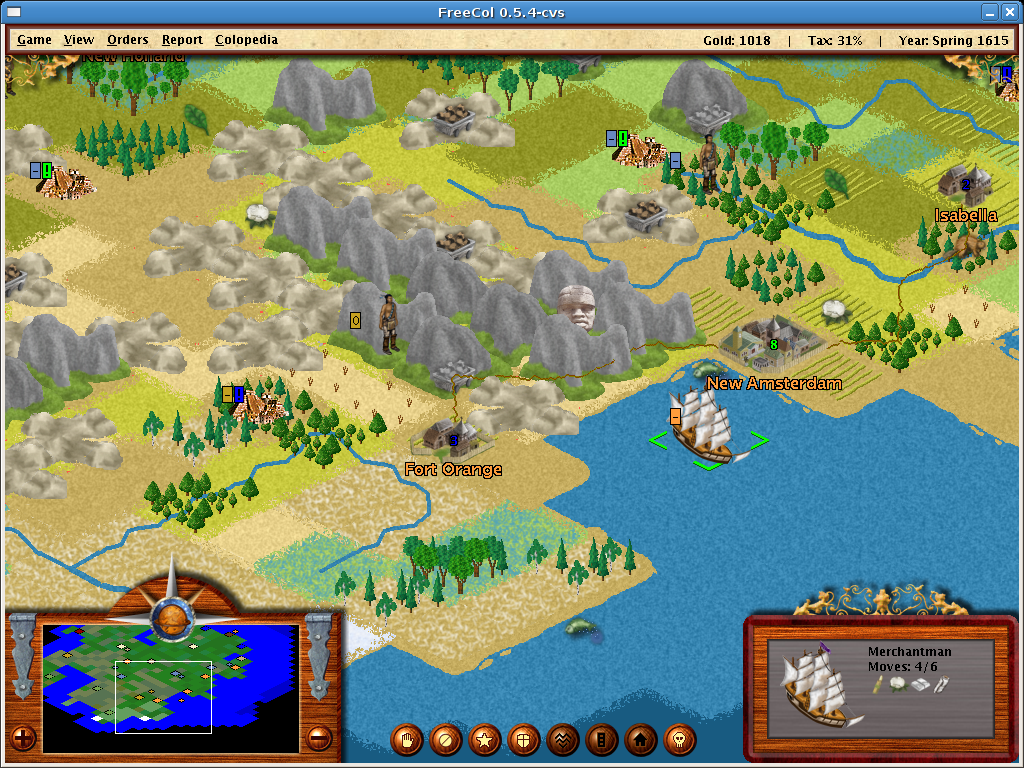
\includegraphics[scale=0.975]{images/main_screen.png}
    \caption{The main screen.\label{main_screen_fig}}
  \end{center}
\end{figure}


In this screen you can see the units, colonies, and so on. You can
move the currently selected unit using the numeric keypad. You can
change the currently selected unit by clicking on an other unit. If
you right click on a tile, you can see the different units that are on
this tile.\\

There are also the following shortcuts:
\begin{itemize}
\item\verb$w$: wait.
\item\verb$space$: skip for this turn.
\item\verb$f$: fortify.
\item\verb$s$: sentry.
\item\verb$p$: plow the current tile.
\item\verb$r$: build a road on the current tile.
\item\verb$b$: build a colony.
%% disband
\item\verb$c$: center on the currently selected unit.
\item\verb$enter$: end the turn.
\item\verb$ctrl-e$: show the Europe panel.
\item\verb$ctrl-t$: show the chat panel.
\item\verb$plus$ or \verb$equals$: zoom in.
\item\verb$minus$ or \verb$underscore$: zoom out.
\item\verb$ctrl-n$: new game.
\item\verb$ctrl-o$: open a game.
\item\verb$ctrl-s$: save a game.
\item\verb$ctrl-r$: reconnect.
\item\verb$ctrl-q$: quit the game.
\item\verb$ctrl-m$: show/hide the map controls.
\item\verb$ctrl-d$: display tile names.
\item\verb$ctrl-g$: display grid.
\end{itemize}

\subsection{The Europe panel}
\label{europe_panel}
The figure \ref{europe_panel_fig} represents the Europe panel.
\begin{figure}
  \begin{center}
    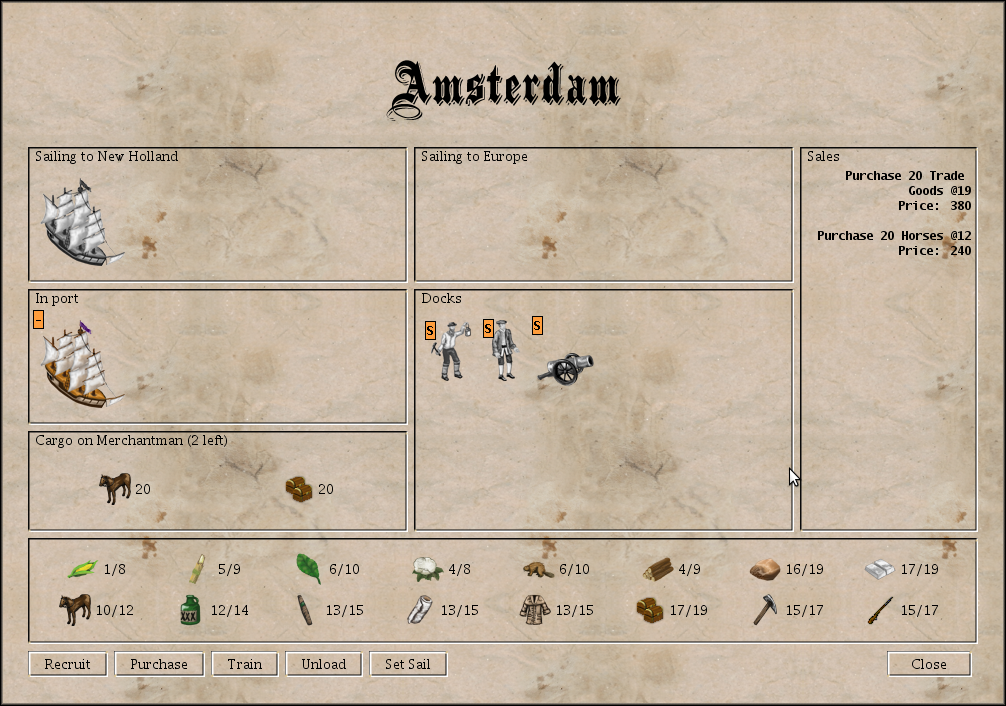
\includegraphics[scale=0.975]{images/europe_panel.png}
    \caption{The Europe Panel.\label{europe_panel_fig}}
  \end{center}
\end{figure}

In this panel, you can control the ships going to Europe, going to
America or being in Europe. You can also buy goods, recruit, purchase
and train units. The units you had recruited, purchased or trained are
in the �Docks� part of the Europe panel.\\

If a ship is going to Europe or going to America, you can drag and
drop it between the two states. If you have a ship in Europe, you can
do the following things:
\begin{itemize}
\item Embark/Disembark units: drag and drop them between the �Docks�
  and �Cargo� parts of the Europe panel.
\item Sell/Buy goods: drag and drop them between the �Cargo� part of
  the Europe panel and the part of the Europe panel where all the
  goods are listed. If you want to sell/buy only a part of a type of
  goods, maintain shift down while dropping it.
\item Arm/Mount/Equip with tools/Dress as missionaries a unit: to do
  that, right click on the unit.
\item Move your ship to the �Going to America� part of the Europe
  panel.
\end{itemize}

\subsection{The Colony panel}
\label{colony_panel}
The figure \ref{colony_panel_fig} represents the Colony panel.
\begin{figure}
  \begin{center}
    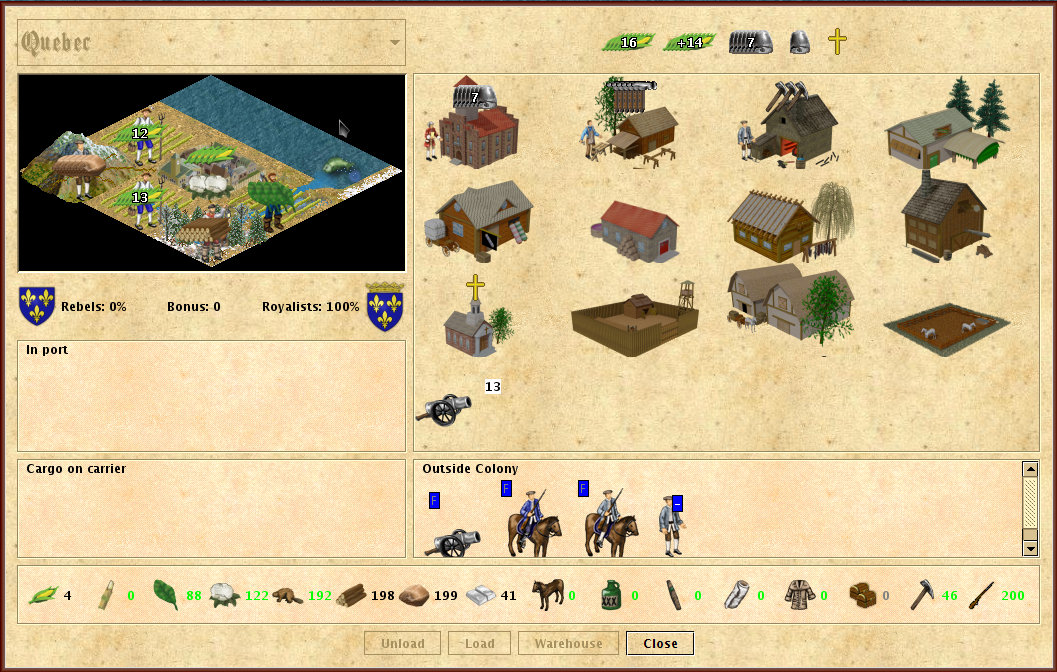
\includegraphics[scale=0.975]{images/colony_panel.png}
    \caption{The Colony Panel.\label{colony_panel_fig}}
  \end{center}
\end{figure}

To view the details about a colony, click on it from the main
screen. The colony panel will then be shown. In this panel, you can
control what your colonists cultivate and produce. You can drag and
drop colonists between the following states:
\begin{itemize}
\item Cultivate something. To do that, drop it into the �Tiles� part of
  the colony panel. You can change what a colonist cultivate by right
  clicking on it.
\item Produce something. To do that, drop it into the �Buildings� part
  of the colony panel.
\item In front of the colony. To do that, drop it into the �In front of
  colony� part of the colony panel.
\item Embark on a ship. If there is a ship in port, you can embark
  your colonist on it by dropping it into the �Cargo� part of the colony
  panel.
\end{itemize}

You can also embark goods on a ship. To do that, drag and drop it into
the �Cargo� part of the colony panel. If you want to embark only a part
of a type of goods, maintain shift down while dropping it.

\end{document}
